\begin{Example}[titanic]{Survival on the \emph{Titanic}}
There have been few marine disasters resulting in the staggering loss of life
than that
which occurred in the sinking of the \emph{Titanic} on April 15, 1912
and (perhaps as a result) few that are so widely known by the public.
It is surprising, therefore, that
neither the exact death toll from this disaster
nor the distributions of death among the passengers
and crew are widely agreed.
\citet[Table 2]{Dawson:95} presents the cross-classification of
2201 passengers and crew on the \emph{Titanic} by Age, Gender, Class
(1st, 2nd, 3rd, Crew) shown in \tabref{tab:titanic} 
(see also \datref{dat:titanic})
and describes his efforts to reconcile various historical sources.
Let us see what we can learn from this \Dset.

%%
%% Table titanic written by md2tex 09APR99 14:57
%%
\begin{table}[htb]
 \caption{Survival on the Titanic}
 \label{tab:titanic}
 \begin{center}
  \begin{tabular}{|lll|rrrr|}
   \hline
 &  &  & \multicolumn{4}{c|}{\bfseries\large Class   }\rule{0in}{2.5ex}\\
{\bfseries\large Gender     } & {\bfseries\large Age     } & {\bfseries\large Survived} & 1st      & 2nd      & 3rd      & Crew     \\
   \hline
Male     & Adult   & Died       &    118 &    154 &    387 &    670 \\
Female   &         &            &      4 &     13 &     89 &      3 \\
[4pt]
Male     & Child   &            &      0 &      0 &     35 &      0 \\
Female   &         &            &      0 &      0 &     17 &      0 \\
[4pt]
Male     & Adult   & Survived   &     57 &     14 &     75 &    192 \\
Female   &         &            &    140 &     80 &     76 &     20 \\
[4pt]
Male     & Child   &            &      5 &     11 &     13 &      0 \\
Female   &         &            &      1 &     13 &     14 &      0 \\
   \hline
  \end{tabular}
 \end{center}
\end{table}


Examining the series of mosaics for the variables ordered
Class, Gender, Age, Survival will show the relationships among
the background variables and how these are related to survival.
The letters $C, G, A, S$ respectively are used to refer to these variables
below.

\figref{fig:mostitanic1} and \figref{fig:mostitanic2}
show the two-way and three-way plots among the background variables.
\figref{fig:mostitanic1} shows that the proportion of males decreases
with increasing economic class, and that the crew was almost entirely male.
The three-way plot (\figref{fig:mostitanic2})
shows the distribution of adults and children among the Class-Gender groups. The
residuals display the fit of a model in which Age is jointly independent of
the Class-Gender categories.
Note that there were no children among the crew, and the overall
proportion of children was quite small (about 5 \%).
Among the passengers, the proportion of children is smallest in
first class, largest in third class.
The only large positive residuals correspond to a greater number of children
among the 3rd class passengers, perhaps representing families traveling
or immigrating together.
%
% subfigmatrix 2 x 1
\begin{figure}[htb]
 \begin{subfigmatrix}{2}
 \subfigure[Class and Gender]{\label{fig:mostitanic1}%
  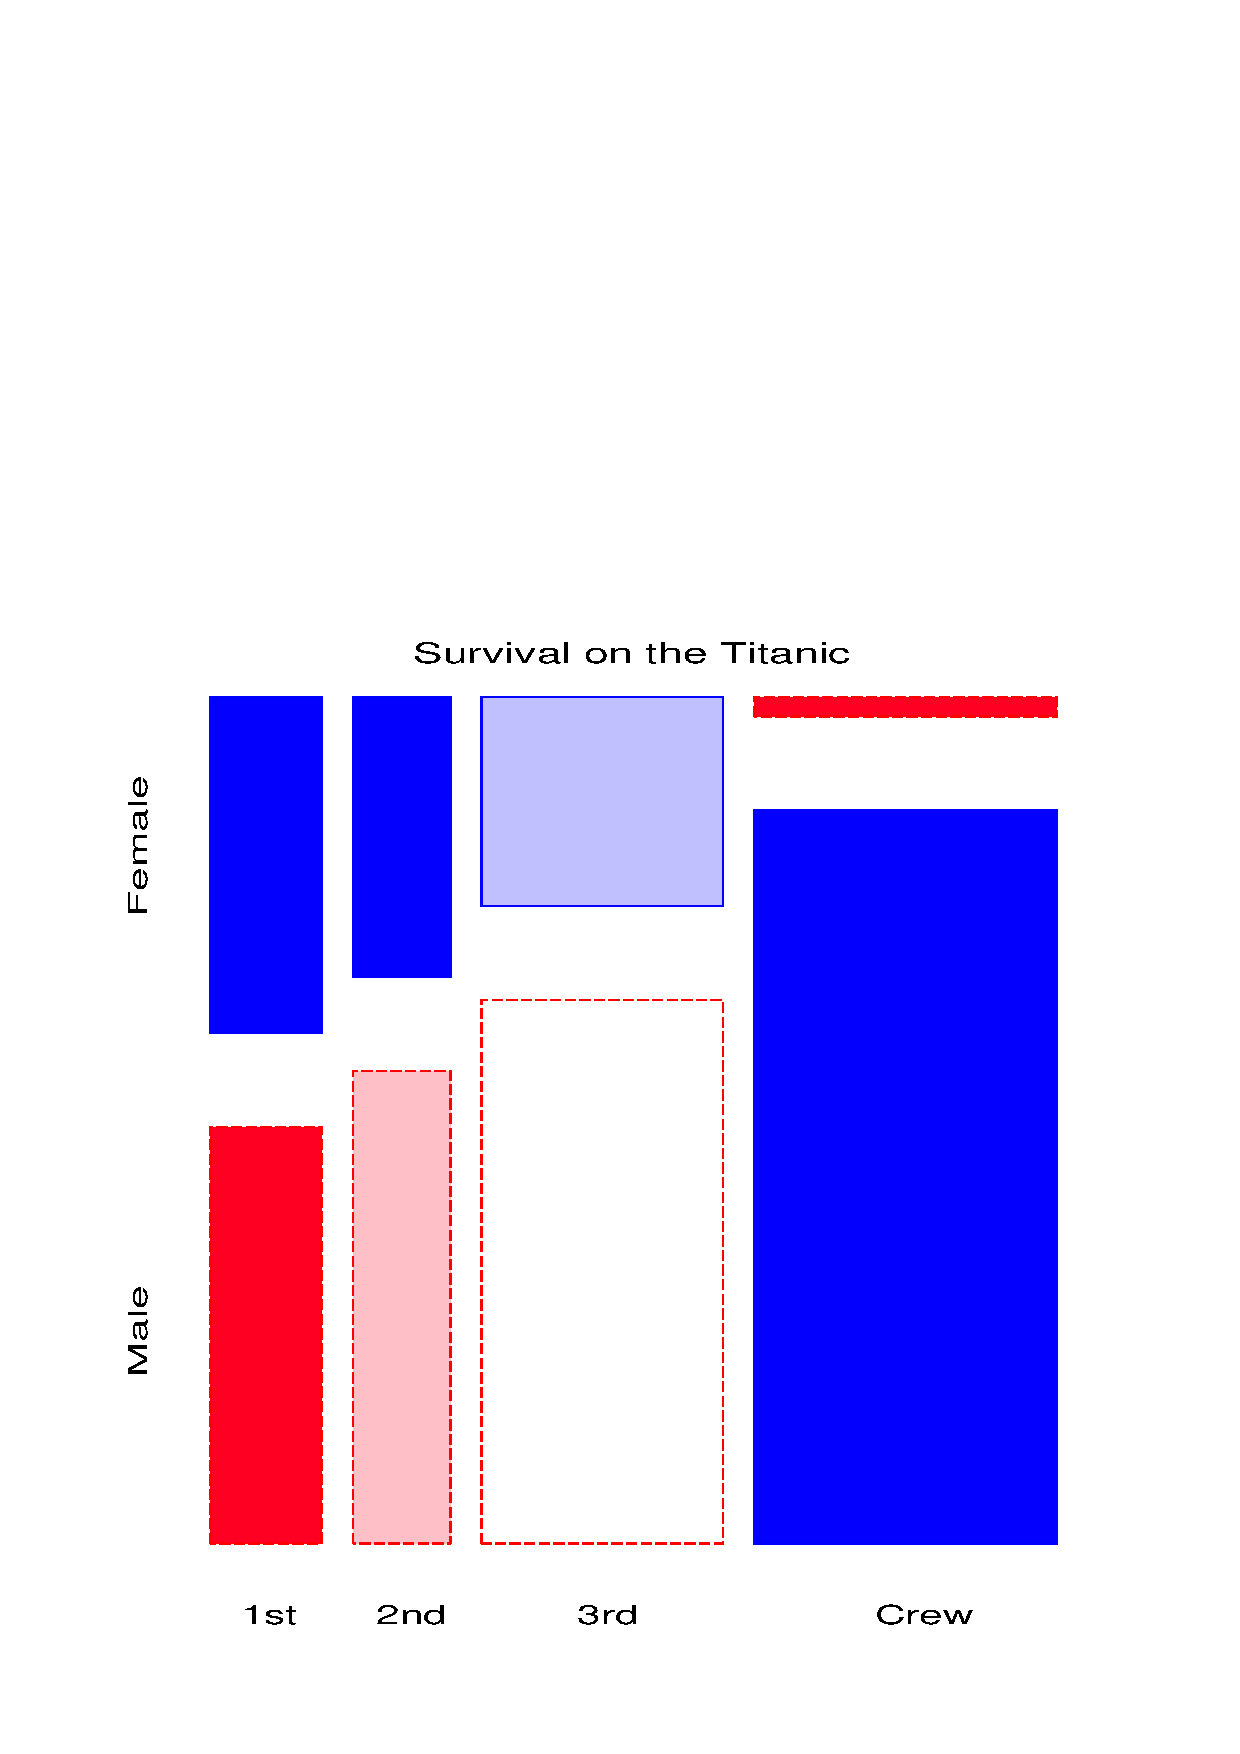
\includegraphics{ch4/fig/mostitanic1}
 }
 \subfigure[Class, Gender, Age]{\label{fig:mostitanic2}%
  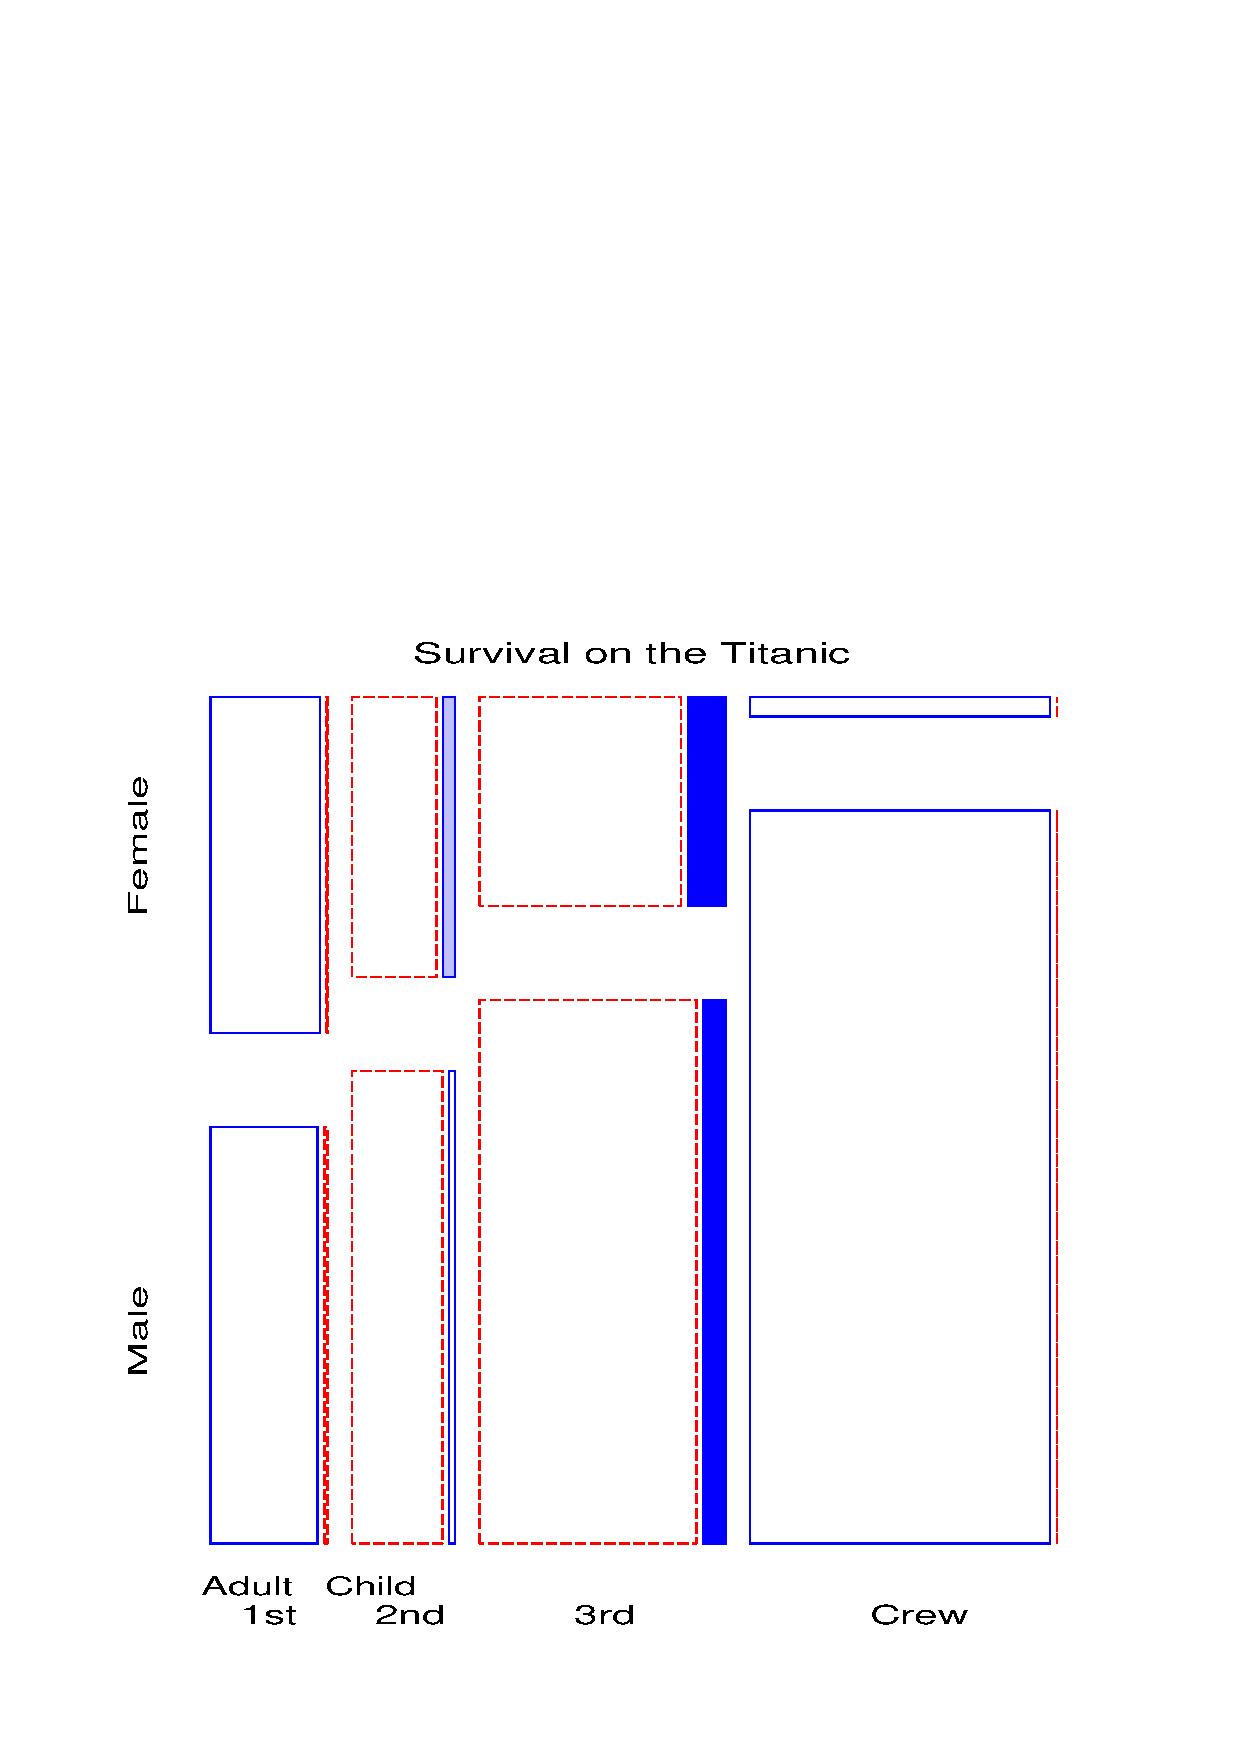
\includegraphics{ch4/fig/mostitanic2}
 }
 \end{subfigmatrix}
 \caption[Titanic data: Background variables]{Titanic data: Background variables}\label{fig:mostitanic1-2}
\end{figure}


The four-way mosaic, shown in \figref{fig:mostitanic3},
fits the model $[CGA][S]$ which asserts that survival is independent
of Class, Gender and Age.
This is the minimal null model when the first three variables are
explanatory.  It is clear that greater proportions of women survived
than men in all classes, but with greater proportions of women surviving
in the upper two classes.  Among males the proportion who survived
also increases with economic class (towards 1st class).
However, this model fits very poorly
($G^2 (15) = 671.96$),
and we may try to fit a more adequate model by adding associations between
survival and the explanatory variables.

Adding an association of each of Class, Gender and Age with Survival
amounts to fitting the model
\LLM{CGA,CS,GS,AS}.  That is, each of the three variables is
associated with survival, but have independent, additive effects. The mosaic for this model is shown in \figref{fig:mostitanic4}.
The fit of this model is much improved ($\Delta G^2 (5) = 559.4$), but still does not represent
an adequate fit ($G^2 (10) = 112.56$).
There are obviously interactions among Class, Gender and Age on their
impact on survival, some of which we have already noted.
%
% subfigmatrix 2 x 1
\begin{figure}[htb]
 \begin{subfigmatrix}{2}
 \subfigure[Joint independence: \LLM{CGA,S}]{\label{fig:mostitanic3}%
  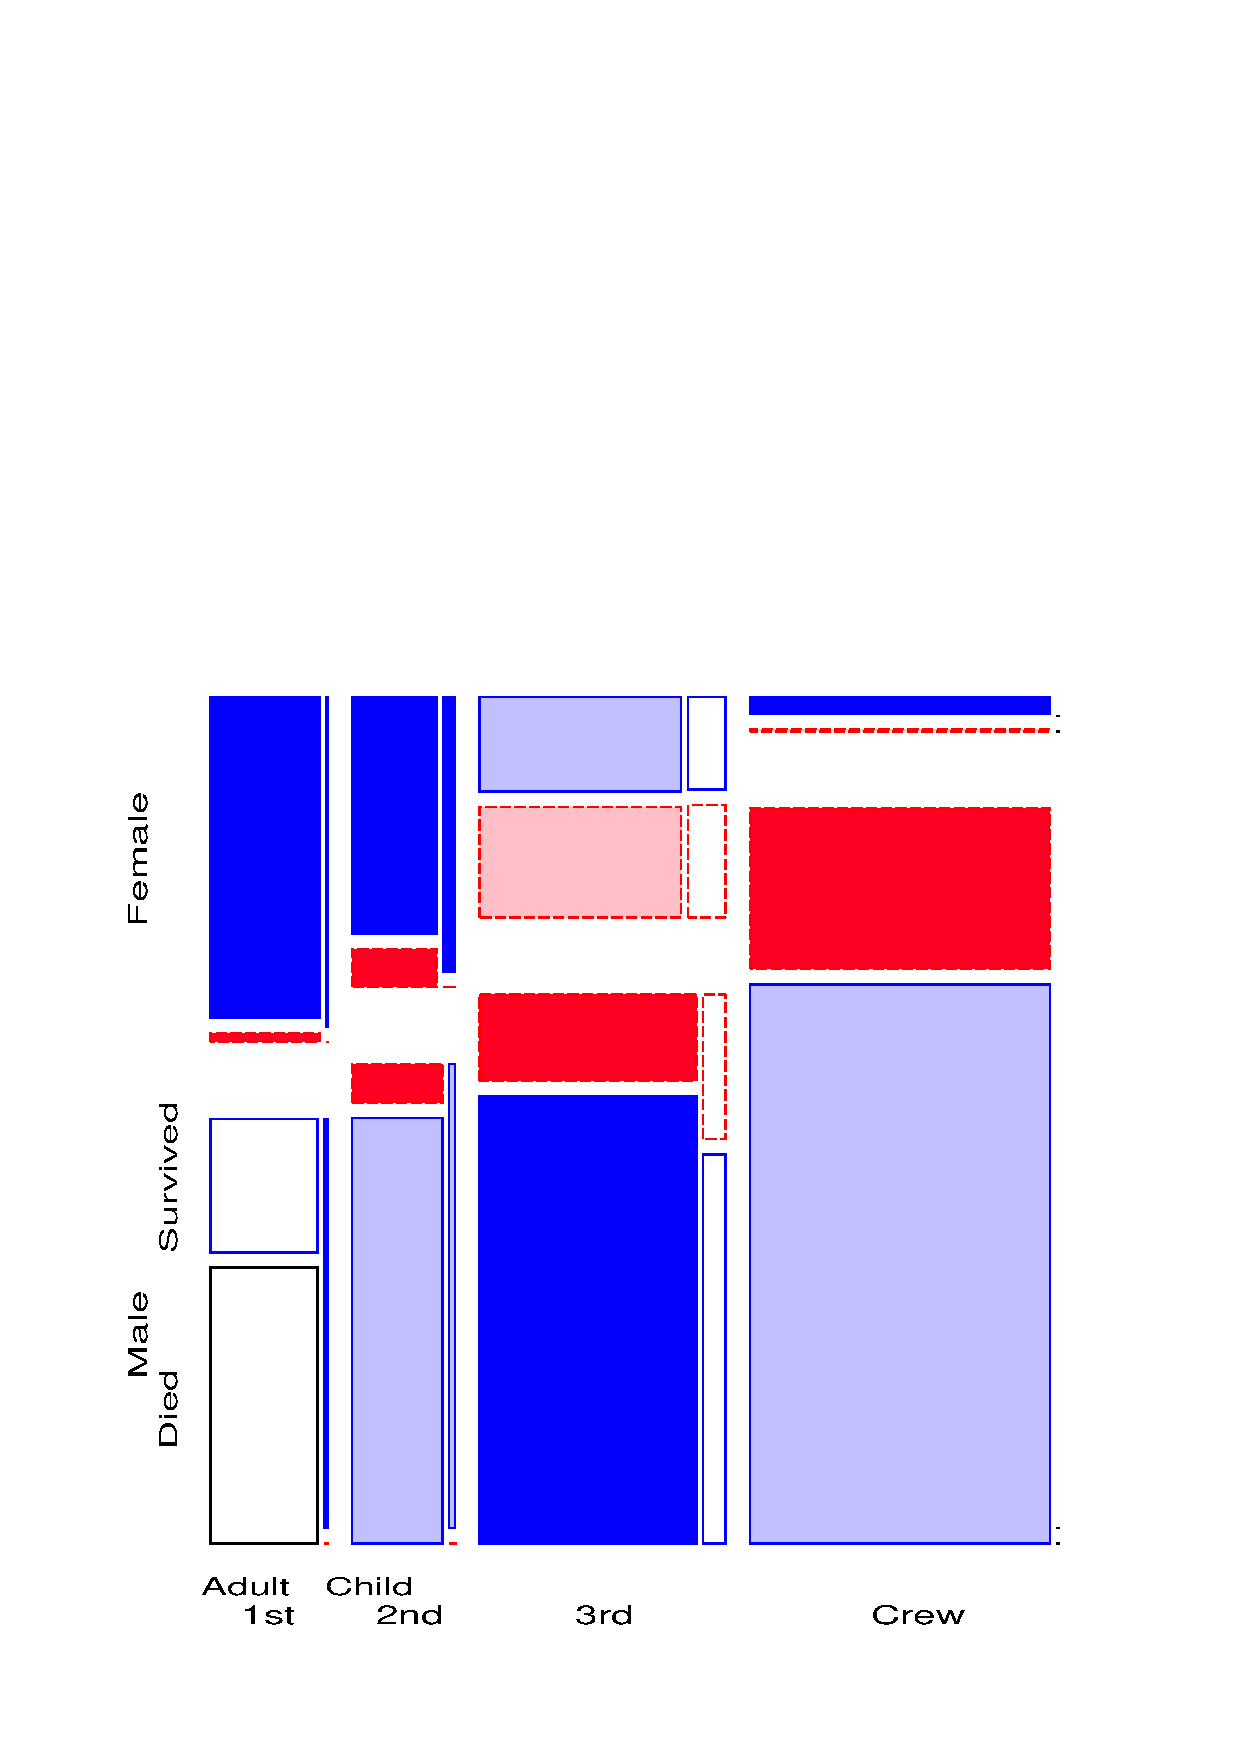
\includegraphics{ch4/fig/mostitanic3}
 }
 \subfigure[Effects of Age, Gender and Class on Survival: \LLM{CGA,CS,GS,AS}]{\label{fig:mostitanic4}%
  \includegraphics{ch4/fig/mostitanic4}
 }
 \end{subfigmatrix}
 \caption[Titanic data: Class, Gender, Age, and Survival]{Titanic data: Class, Gender, Age, and Survival}\label{fig:mostitanic3-4}
\end{figure}
%

Taking the rubric of ``women and children first,'' we next fit the
model \LLM{CGA,CS,GAS} in which Age and Gender interact in their influence
on survival.  The mosaic for this model is shown in \figref{fig:mostitanic5}.
Adding the association of Age and Gender with survival has
improved the model slightly, however the fit is still not good ($G^2 (9) = 94.54$).
If we add the interaction of Class and Gender to this
(the model \LLM{CGA,CGS,GAS}) the \LR{} chi-square is reduced
substantially ($G^2 (6) = 37.26$), but the lack of fit is still
significant.

Finally, we try a model in which Class interacts with both
Age and Gender to give the model
\LLM{CGA,CGS,CAS}, whose residuals are shown in \figref{fig:mostitanic6}.
The \LR{} chi-square is now 1.69 with 4 df, a very good fit, indeed.
%
% subfigmatrix 2 x 1
\begin{figure}[htb]
 \begin{subfigmatrix}{2}
 \subfigure[Model \LLM{CGA,CS,GAS}]{\label{fig:mostitanic5}%
  \includegraphics{ch4/fig/mostitanic5}
 }
 \subfigure[Model \LLM{CGA,CGS,CAS}]{\label{fig:mostitanic6}%
  \includegraphics{ch4/fig/mostitanic6}
 }
 \end{subfigmatrix}
 \caption[Titanic data: Models with interactions]{Titanic data: Models with interactions}\label{fig:mostitanic5-6}
\end{figure}

The import of these figures is clear.
Regardless of Age and Gender, lower economic
status was associated with increased mortality; the differences due to Class
were moderated, however, by both Age and Gender.
Although women on the \emph{Titanic}
were more likely overall
to survive than men, the interaction of Class and Gender shows that
women in 3rd class did not have a significant advantage, while men in 1st class
did compared to men in other classes.  The interaction of Class and
Age is explained by the observation
that while no children in 1st or 2nd class died,
nearly two-thirds in 3rd class died;
for adults, mortality increases progressively
as economic class declines.
Hence, although the phrase ``women and
children first'' is mellifluous and appeals to our sense of Edwardian chivalry
a more adequate description might be
``women and children (according to class), then 1st class men.''
\end{Example}
